\documentclass[twoside]{article}
\setlength{\oddsidemargin}{0.25 in}
\setlength{\evensidemargin}{-0.25 in}
\setlength{\topmargin}{-0.6 in}
\setlength{\textwidth}{6.5 in}
\setlength{\textheight}{8.5 in}
\setlength{\headsep}{0.75 in}
\setlength{\parindent}{0 in}
\setlength{\parskip}{0.1 in}

\usepackage{graphicx}
\usepackage{url}
\usepackage{listings}
\usepackage{color}
\usepackage{svg}

%
% The following commands sets up the lecnum (lecture number)
% counter and make various numbering schemes work relative
% to the lecture number.
%
\newcounter{lecnum}
\renewcommand{\thepage}{\thelecnum-\arabic{page}}
\renewcommand{\thesection}{\thelecnum.\arabic{section}}
\renewcommand{\theequation}{\thelecnum.\arabic{equation}}
\renewcommand{\thefigure}{\thelecnum.\arabic{figure}}
\renewcommand{\thetable}{\thelecnum.\arabic{table}}
\newcommand{\dnl}{\mbox{}\par}

%
% The following macro is used to generate the header.
%
\newcommand{\lecture}[4]{
  \pagestyle{myheadings}
  \thispagestyle{plain}
  \newpage
  \setcounter{lecnum}{#1}
  \setcounter{page}{1}
  \noindent
  \begin{center}
  \framebox{
     \vbox{\vspace{2mm}
   \hbox to 6.28in { {\bf COMPSCI~590S~~~Systems for Data Science
                       \hfill Fall 2017} }
      \vspace{4mm}
      \hbox to 6.28in { {\Large \hfill Lecture #1: #2  \hfill} }
      \vspace{2mm}
      \hbox to 6.28in { {\it Lecturer: #3 \hfill Scribe(s): #4} }
     \vspace{2mm}}
  }
  \end{center}
  \markboth{Lecture {#1}: #2}{Lecture {#1}: #2}
  \vspace*{4mm}
}

%
% Convention for citations is authors' initials followed by the year.
% For example, to cite a paper by Leighton and Maggs you would type
% \cite{LM89}, and to cite a paper by Strassen you would type \cite{S69}.
% (To avoid bibliography problems, for now we redefine the \cite command.)
%
\renewcommand{\cite}[1]{[#1]}

% \input{epsf}

%Use this command for a figure; it puts a figure in wherever you want it.
%usage: \fig{NUMBER}{FIGURE-SIZE}{CAPTION}{FILENAME}
\newcommand{\fig}[4]{
           \vspace{0.2 in}
           \setlength{\epsfxsize}{#2}
           \centerline{\epsfbox{#4}}
           \begin{center}
           Figure \thelecnum.#1:~#3
           \end{center}
   }

% Use these for theorems, lemmas, proofs, etc.
\newtheorem{theorem}{Theorem}[lecnum]
\newtheorem{lemma}[theorem]{Lemma}
\newtheorem{proposition}[theorem]{Proposition}
\newtheorem{claim}[theorem]{Claim}
\newtheorem{corollary}[theorem]{Corollary}
\newtheorem{definition}[theorem]{Definition}
\newenvironment{proof}{{\bf Proof:}}{\hfill\rule{2mm}{2mm}}

% Some useful equation alignment commands, borrowed from TeX
\makeatletter
\def\eqalign#1{\,\vcenter{\openup\jot\m@th
 \ialign{\strut\hfil$\displaystyle{##}$&$\displaystyle{{}##}$\hfil
     \crcr#1\crcr}}\,}
\def\eqalignno#1{\displ@y \tabskip\@centering
 \halign to\displaywidth{\hfil$\displaystyle{##}$\tabskip\z@skip
   &$\displaystyle{{}##}$\hfil\tabskip\@centering
   &\llap{$##$}\tabskip\z@skip\crcr
   #1\crcr}}
\def\leqalignno#1{\displ@y \tabskip\@centering
 \halign to\displaywidth{\hfil$\displaystyle{##}$\tabskip\z@skip
   &$\displaystyle{{}##}$\hfil\tabskip\@centering
   &\kern-\displaywidth\rlap{$##$}\tabskip\displaywidth\crcr
   #1\crcr}}
\makeatother

% **** IF YOU WANT TO DEFINE ADDITIONAL MACROS FOR YOURSELF, PUT THEM HERE:

\definecolor{dkgreen}{rgb}{0,0.6,0}
\definecolor{gray}{rgb}{0.5,0.5,0.5}
\definecolor{mauve}{rgb}{0.58,0,0.82}

\lstset{frame=tb,
  language=Python,
  aboveskip=3mm,
  belowskip=3mm,
  showstringspaces=false,
  columns=flexible,
  basicstyle={\small\ttfamily},
  numbers=none,
  numberstyle=\tiny\color{gray},
  keywordstyle=\color{blue},
  commentstyle=\color{dkgreen},
  stringstyle=\color{mauve},
  breaklines=true,
  breakatwhitespace=true,
  tabsize=3
}

% Some general latex examples and examples making use of the
% macros follow.

\begin{document}

%FILL IN THE RIGHT INFO.
%\lecture{**LECTURE-NUMBER**}{**DATE**}{**LECTURER**}{**SCRIBE**}
\lecture{11}{FlumeJava, Memory Allocation and Garbage Collection}{Emery Berger}{Anmol Singh Suag, Cen Wang}

Last time, we talked about the widespread usage of JVM languages (Java, Scala, Clojure, Kotlin, etc.) in big data area. JVM has the advantages of:

\begin{enumerate}
\item Garbage collection makes it easy to write correct programs.
\item JVM’s JIT compiler is optimized so that JVM has high performance.
\end{enumerate}

JIT startup time is a little concerning, but if our program will keep running for a long time then the cost is amortized.

\section{FlumeJava}

Because memory is much faster than disks and networks, we'd like to do as much computation as possible in RAM to minimize IO cost. For a MapReduce stage, both the map result and the reduce result have to be written to disk or GFS (which is network IO). If the problem at hand (e.g. wordcount in MapReduce) requires only one MapReduce stage, this IO cannot be avoided. But usually, real life problems requires a pipeline of MapReduce jobs, meaning that multiple stages of MapReduce will be started. A typical example will be running stochastic gradient descent algorithm in MapReduce.

\begin{lstlisting}
epsilon = 0.0001
last_result # Stores result for last iteration
while True:
    result = do_some_mapreduce_job()
    if last_result - result <= epsilon: # The result has converged
        break
\end{lstlisting}

In the above example, multiple MapReduce jobs will be started until we reach the convergence condition. In this situation, IO cost between the previous and the current MapReduce slows the entire computation down. FlumeJava's idea is that instead of starting multiple MapReduce phases, we can first try to optimize the computation process so that IO costs can be reduced.

The FlumeJava library does this by deferring the actual computation to a later time. When the user is defining a series of transformation of the data, there is actually no real computation happening in the MapReduce cluster. Instead, FlumeJava secretly constructs a computation graph (or dataflow graph) of the transformation. The dataflow graph exposes opportunities to optimize the computation process, saving the unnecessary MapReduce phases and thus saves IO and time. The FlumeJava library works in the following way:

\begin{enumerate}
\item Defer the computation and construct dataflow graph
\item Optimize the dataflow graph
\item Execute the optimized dataflow graph
\end{enumerate}

For example, if we are going to transform data first by function f and then by function g, a handwritten MapReduce pipeline will be:

\begin{lstlisting}
y = mapreduce(f(x))
# A lot of IO happening here to save the result
z = mapreduce(g(y))
# A lot of IO happening here to save the result
\end{lstlisting}

The FlumeJava library will first draw a computation graph and then notice that the intermediate result y is used immediately after the first MapReduce job, so it will fuse the two MapReduce jobs into one:

\begin{lstlisting}
mapreduce(g(f(x)))
# A lot of IO happening here to save the result
\end{lstlisting}

This saves one unnecessary IO phase. FlumeJava’s strategy can also be referred as lazy evaluation, which is different from a handwritten MapReduce pipeline’s eager evaluation where there will be no opportunities for optimization.

There is a tradeoff between eager and lazy evaluation.

\begin{enumerate}
	\item Lazy evaluation: suitable for \textbf{batch processing}
    \begin{enumerate}
		\item - Higher latency
        \item + Higher throughput
	\end{enumerate}
	\item Eager evaluation: suitable for \textbf{stream processing, to be discussed}
    \begin{enumerate}
		\item + Lower latency
        \item - Lower throughput
	\end{enumerate}
\end{enumerate}

\section{Memory Management}
In C/C++, programmers have to manually manage their memory.

C: new/malloc

C++: delete/free

Manual memory management is risky. Many kinds of security problems have been discovered to be related to manual memory management.

\subsection{Memory allocator}

A traditional memory allocator is called bump pointer allocation. When you call sbrk(8), you can get 8 bytes of heap memory, and a pointer pointing to where the heap used to be will be returned.

\subsection{Memory utilization}

Imagine we have the following program:

\begin{lstlisting}
for (int i = 0; i < 10000000; i++) {
    void* p = malloc(8);
    // Do something here
    free(p);
}
\end{lstlisting}

It first requests 8 bytes of memory, does some computation, and then free the that 8 bytes. This program needs at most 8 bytes of heap memory. Then consider the following naive memory allocator implementation:

\begin{lstlisting}
void* malloc(size_t size) {
    return sbrk(size);
}

void free(void* p) {
    // Do nothing
}
\end{lstlisting}

What this memory allocator does is that it give whatever size of memory the user want but it never tries to free any memory. If we use the above naive memory allocator, then our memory consumption goes linearly with the time but the actually memory needed is only 8 bytes. There is a large amount of the memory being wasted with this memory allocator. We can think with the following formula:

Fragmentation = (memory consumed by allocator - memory requested by user) / memory requested by user

An ideal allocator would be that the allocator only consumes the amount of memory requested by the user. In this case, fragmentation is 0.

\subsection{Memory fragmentation}

\subsubsection{Internal fragmentation (means memory is wasted inside the allocated object)}

Modern processors usually can only access the memory at the granularity and alignment of their word size, known as alignment restriction. If memory is misaligned, the system may have a poor performance. Because of this, when you try to request 1 byte of heap memory by malloc(1), Linux operating system will actually allocate 8 bytes of memory for you to meet the alignment requirement. The extra 7 bytes of memory is wasted inside the object.

A second form of internal fragmentation is memory bookkeeping. In Linux, another 8 bytes of heap metadata is attached for every object that is allocated. Notice that when we free heap memory by free(p), we don’t have to specify how many bytes we want to free. This information is actually bookkept in heap metadata, so when the operating system receive a request to free some part of the memory, it only needs to look ahead 8 bytes to the place where the metadata is stored, then it knows how many bytes to free.

Pros and cons:

\begin{enumerate}
\item + Cheap implementation
\item - Space utilization
\item - Cache utilization
\item - Security
\end{enumerate}

BiBoP allocator

An alternative allocation strategy is BiBoP. The allocator creates different pages for different sizes of objects. So there may be 8-byte, 16-byte, 32-byte object page. At the beginning of the page, there is a pointer pointing to other memory address where the page metadata is stored such as size. So when we allocate for new objects, those objects of the same size go to the same page. When we do free(p), under the hood, we will first find the pointer at the beginning of the page and then follow the pointer to get the page metadata which is the same for every object in that page.

\subsubsection{External fragmentation (means memory is wasted outside the allocated object or between allocated objects)}

Imagine we have 8 bytes of memory:

\begin{lstlisting}
----------
|________|
\end{lstlisting}

We first request 1 byte of memory eight times (suppose we do not have alignment restriction here):

\begin{lstlisting}
----------
|xxxxxxxx|
----------
\end{lstlisting}

Then we free the first, third, fifth and seventh allocation:

\begin{lstlisting}
----------
| x x x x|
----------
\end{lstlisting}

At this time, we have 4 bytes of free memory. But even if the space is there, the program cannot even allocate a 2-byte memory. This phenomenon is known as external fragmentation. 

One solution to this problem is compaction. We can compact the above memory to eliminate external fragmentation:

\begin{lstlisting}
----------
|xxxx____|
\end{lstlisting}

We can now allocate a 2-byte memory. Memory compaction has high cost, as you have to move objects and edit the pointers. Also, this is not doable in C/C++.

\section{Garbage Collection}
C/C++ are not ‘type-safe’ and they don’t differentiate between pointers and data. If data addresses were to be changed, the pointer algorithms would fail. Hence, compaction and garbage collection doesn’t work with C/C++, memory has to be manually freed.

There are 2 reasons why Garbage Collection is interesting :
It is easy and safe; There is no manual deleting required of unused objects
It prevents memory fragmentation through memory compaction

LISP was the first language to be shipped with in-built Garbage Collectors around 1960.

There are 2 Garbage Collection Algorithms:

\subsection{Reference Counting}

Reference Counting is a very simple algorithm, but has a fundamental problem. In this algorithm, each object maintains a count of the number of pointers that are pointing to it. This count is called its Reference Count. The object is immediately deleted by the algorithm when its Reference Count becomes 0.

Say, for eg:

\begin{lstlisting}
P = new(X)
Q = P
R = P
\end{lstlisting}

The object X now has a Reference Count of 3.

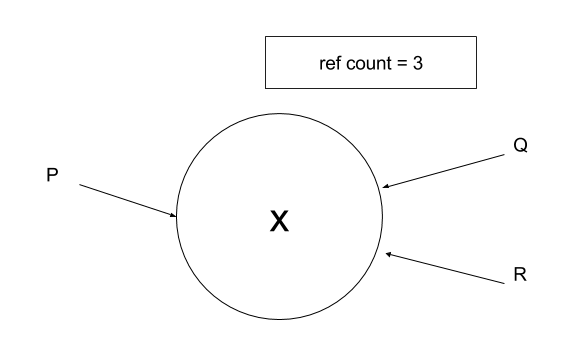
\includegraphics[width=100mm,scale=0.5]{1.png}

Now say we perform:

\begin{lstlisting}
Q = null  // Ref Count = 2
R = null  // Ref Count = 1
P = null  // Ref Count = 0 and X is deleted by the algorithm
\end{lstlisting}

X is deleted as soon as its Reference count drops to 0.

Developing further on the previous example, say X points to another object Y that points to another object Z and so on. The Reference Counts can be showed as follows:

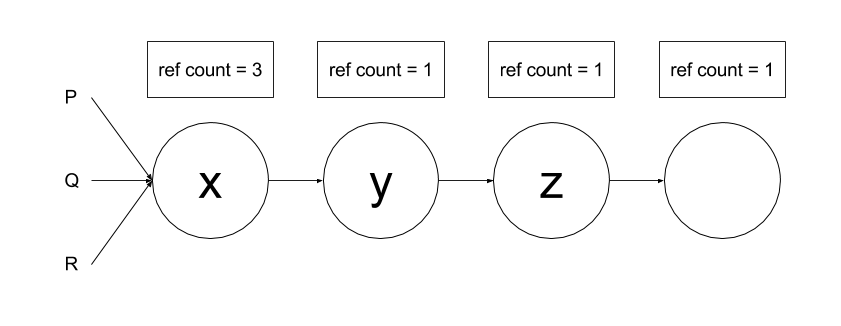
\includegraphics[width=150mm,scale=0.5]{2.png}

When P,Q are R are set to null, the Reference Count of X becomes 0 and it is deleted. Hence, the Reference Count of Y becomes 0 and it is deleted as well. Similarly, Z and so on are deleted by the Reference Counting Garbage Collector.

This seems like a great approach! Reference Counting was developed in the 1950s and was used in LISP. It was also adopted in Perl.

Reference Counting algorithm is:

\begin{enumerate}
\item Super Easy ( + )
\item Immediate  ( + )
\item Incomplete ( - )
\end{enumerate}

Reference count garbage collector can reclaim a piece of memory only when that piece of memory’s reference count reaches 0. It is incomplete in its fundamental nature. The following figure explains the problem:

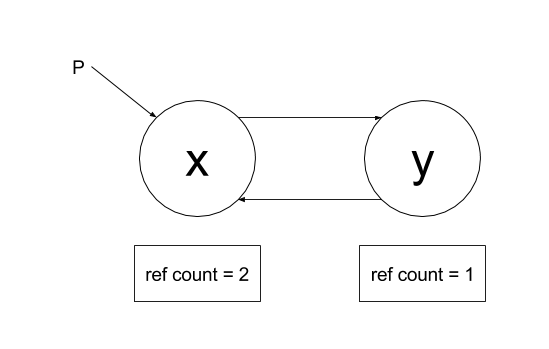
\includegraphics[width=100mm,scale=0.5]{3.png}

Object X has a Reference Count of 2 and Y has a Reference Count of 1. When P is marked as null, we are left with a cycle where X and Y point to each other and hence have Reference Counts of 1 each. This cycle would not be deleted by the algorithm as their Reference Counts are not 0. Such cycles are called ‘Reference Cycles’.

Memory can not be reclaimed from cycles by Reference Counting Garbage Collector even if they are not reachable from the outside world. Avoiding cycles is hard; Like Doubly Linked-Lists have a forward and backward pointers for each node. This is the reason Perl servers have to be periodically restarted; dumping everything and starting afresh is an easy work-around.

The other garbage collecting algorithm that can detect cycles is Mark-And-Sweep.

\subsection{Mark-And-Sweep}

The Mark-And-Sweep Garbage Collector follows a simple rule : ‘Objects that are unreachable by pointers are garbage’. The algorithm considers reachability of an object to detect its aliveness.

Every object has a ‘Mark Bit’. Starting from the globals, stack and registers ( the roots ) , the algorithm follows the paths along the pointers to mark all the objects it crosses as ‘black’.

\begin{lstlisting}
Mark(P) {
	if( Markbit (P) == White ) {
		Markbit (P) = Black }
	Mark( All_Outgoing_Links)  ⇒ Recursion
	}
\end{lstlisting}

Eventually, all reachable ( alive ) objects are marked as ‘Black’. This is the Mark phase of the algorithm.  All objects that remain marked as ‘White’ are considered to be garbage and are deleted in the ‘Sweep’ phase.

Mark-And-Sweep is a complete algorithm that is guaranteed to free all garbage. It is a ‘deferred collection’ algorithm and may result in big pauses.

\begin{enumerate}
\item + Complete
\item - Deferred Collection
\item - Big Pause
\end{enumerate}

Garbage collection is computationally expensive and involves a lot of operations. If Garbage Collection was to be triggered after every operation, it would slow down the throughput of the machine by a huge margin. Therefore, Mark-And-Sweep does a Deferred Collection. 

1 Op $\rightarrow$ 1 Billion Ops for GC $\rightarrow$ 1 Op $\rightarrow$ 1 Billion Ops for GC $\Rightarrow$ Not Good

1 Billion Ops $\rightarrow$ 1 Billion Ops for GC $\Rightarrow$ Good

We want to accumulate garbage for some while and then clean them to amortize the GC cost rather than start GC every operation.

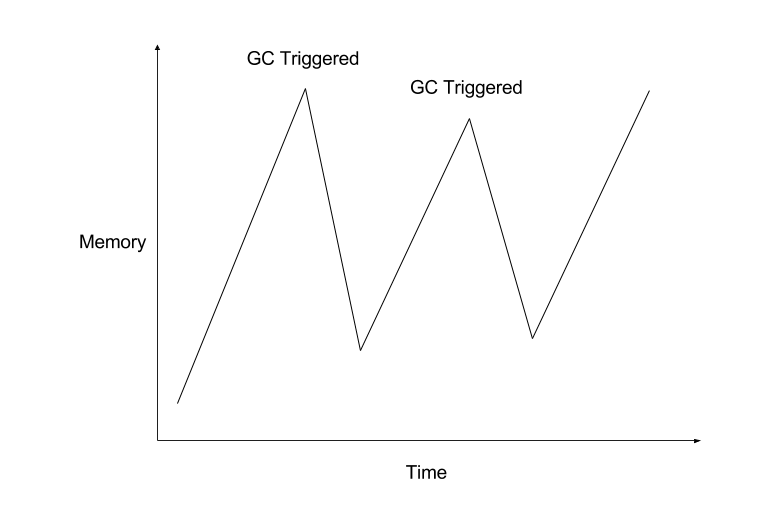
\includegraphics[width=150mm,scale=0.5]{4.png}

As we chose to defer Garbage Collection and let garbage accumulate while immediately getting more memory as long it lasts, we have to keep a lot of extra memory to accommodate the alive and dead objects until the collection happens. This wastes a lot of memory and results in poor memory utilization. Maximising Memory Utilization is desirable. In C, C++ and MapReduce if you need 1 GB memory, you use just 1 GB memory. Hence, the memory utilization is 1. In Java with Garbage Collection, to use 1 GB memory, you need about 3-5 GB memory. Therefore the utilization is quite small.

\begin{center}
    \begin{tabular}{ | l | l | l | l |}
    \hline
    Memory Used & Memory Needed & Utilization & Examples \\ \hline
    1 GB & 1 GB & 1 & C, C++, MapReduce \\ \hline
    1 GB & about 3-5 GB & 1/3 to 1/5 & GC, Java, Hadoop \\
    \hline
    \end{tabular}
\end{center}

\end{document}